\documentclass[DIV16,BCOR1cm,10pt,a4paper,fleqn,twoside]{scrreprt}         % for pdf output
%\documentclass[DIV16,BCOR1cm,10pt,a4paper,fleqn]{scrreprt}         % for pdf output
%\documentclass[DIV16,BCOR1cm,11pt,a4paper,fleqn]{report}         % for pdf output

% To allow automatic selection of the right graphics type ...
% preset \pdfoutput for older latex installation, it is allways definted for
% news ones
\ifx\pdfoutput\undefined
\gdef\pdfoutput{0}
\fi

\newif\ifpdfx
\ifnum\pdfoutput=0
% latex is called for dvi output
   \pdfxfalse
   \usepackage{graphicx}
\else
% pdflatex is called for pdf output
   \pdfxtrue
   \usepackage[pdftex]{graphicx}
   \usepackage[pdftex]{hyperref}
\fi

\usepackage{textcomp}


\usepackage{transparent}
\usepackage{eso-pic}
\newcommand\BackgroundPic{%
\put(0,0){%
\parbox[b][\paperheight]{\paperwidth}{%
\vfill
\centering
{\transparent{1.0} \includegraphics[width=16cm,height=\paperheight,%
keepaspectratio]{cdo_libdep.pdf}}%
\vfill
}}}

%\newcommand{\CDO}{{\bfseries\sffamily CDO\ }}
\newcommand{\CDO}{{\bfseries\sffamily CDO}}
\newcommand{\cdologo}{
\includegraphics{logo/cdo_logo}}

\graphicspath{{figures/}}

% To define headers and footers
\usepackage{fancyhdr}
\pagestyle{fancy}

% Headers and footers personalization using the `fancyhdr' package
\fancyhf{} % Clear all fields

\renewcommand{\headrulewidth}{0.2mm}
\renewcommand{\footrulewidth}{0.2mm}

\renewcommand{\chaptermark}[1]{\markboth{#1}{}}
\renewcommand{\sectionmark}[1]{\markright{#1}}

%\renewcommand{\chaptermark}[1]{\markboth{#1}{}}
%\renewcommand{\sectionmark}[1]{\markleft{#1}}

\fancyhead[LO,RE]{\slshape \leftmark}
\fancyhead[LE,RO]{\slshape \rightmark}
\fancyfoot[LE,RO]{\Large\thepage}
%\fancyfoot[LO,RE]{\raisebox{-2.8mm}{\scalebox{0.17}{\cdologo}}}
\fancypagestyle{plain}{%
  \fancyhead{} % get rid of headers
  \renewcommand{\headrulewidth}{0pt}
}

%\setlength{\footnotesep}{0cm}
%\setlength{\footskip}{-2cm}
%\renewcommand{\footnoterule}{\rule{0cm}{0cm}}

\usepackage{multirow}

\usepackage[T1]{fontenc}
\usepackage[lighttt]{lmodern}

\usepackage{exscale}
\usepackage{array,colortbl}    % color table

\usepackage{listings}
\usepackage{longtable}
\usepackage{color}
\definecolor{pcolor1}{rgb}{0.992, 0.980, 0.875}  % rgb: 253/250/223
\definecolor{pcolor2}{rgb}{1.000, 0.925, 0.700}  % rgb: 255/236/278
\definecolor{pcolor3}{rgb}{0.968, 0.756, 0.623}  % rgb: 247/193/159

%\usepackage{ae}               % fuer die "almost european" computer modern fonts
%\usepackage{url}              % Standard-Paket fuer WWW-Adressen

%\typearea{10}                 % Einen sinnvollen Satzspiegel aktivieren


%Usage:
%pdflatex cdo.tex
%pdflatex cdo.tex
%cat > cdo.ist << 'EOF'
%delim_0        "{\\idxdotfill} "
%headings_flag  1
%heading_prefix "{\\centerline {\\Large \\textbf{"
%heading_suffix "}}}"
%EOF
%makeindex -s cdo.ist cdo.idx
%pdflatex cdo
%thumbpdf cdo
%pdflatex cdo


\usepackage{thumbpdf}

%\usepackage{html}

\usepackage{makeidx}

%\ifpdf
%\usepackage[a4paper, colorlinks=true, pdfstartview=FitV, bookmarks=true, linkcolor=blue,
%            citecolor=blue, urlcolor=blue, latex2html=true]{hyperref}
%\fi

\usepackage{hyperref}
\hypersetup{pdftoolbar=true,
            pdfmenubar=true,
            pdfwindowui=true,   
%            pdffitwindow=true,
            pdfauthor={Uwe Schulzweida},
            pdftitle={CDO Climate Data Operators},
            pdfcreator={pdflatex + hyperref},
            pdfstartview=FitV,
%            pdfpagemode=FullScreen,
            a4paper,
            bookmarks=true,
            linkcolor=blue,
            citecolor=blue,
            urlcolor=blue,
            colorlinks=true}

\setlength{\parindent}{0em}
\setlength{\parskip}{1.5ex plus0.5ex minus0.5ex}
\extrarowheight1pt

\makeindex
%\newcommand{\ii}[1]{\textit{#1}}  \newcommand{\nn}[1]{#1n}
%\renewcommand{\dotfill}{\leaders\hbox to 5p1{\hss.\hss}\hfill}
%\newcommand{\idxdotfill}{5p1{\hss.\hss}\hfill}
\newcommand{\idxdotfill}{\ \dotfill \ }
%\def\idxdotfill{\leaders\hbox to.6em{\hss .\hss}\hskip 0pt plus 1fill}
%\MakeShortVerb{\@}

\renewcommand{\indexname}{Operator index}

\newenvironment{defalist}[1]
{\begin{list}{}
{\settowidth{\labelwidth}{#1\ \ }
\setlength{\itemsep}{0mm}
\setlength{\itemindent}{0mm}
%\setlength{\listparindent}{25mm}
\setlength{\leftmargin}{\labelwidth}
%\setlength{\leftmargin}{25mm}
\setlength{\labelsep}{2mm}
\addtolength{\leftmargin}{\labelsep}
%\addtolength{\leftmargin}{8mm}
}}
{\end{list}}

\newenvironment{defalist2}[1]
{\begin{list}{}
{\settowidth{\labelwidth}{#1\ \ }
\setlength{\itemsep}{0mm}
\setlength{\itemindent}{0mm}
%\setlength{\listparindent}{25mm}
\setlength{\leftmargin}{\labelwidth}
%\setlength{\leftmargin}{25mm}
\setlength{\labelsep}{2mm}
\addtolength{\leftmargin}{\labelsep}
\addtolength{\leftmargin}{8mm}
}}
{\end{list}}

\newcommand{\miniwidth}{\textwidth}

\setcounter{secnumdepth}{3}

\begin{document}

% \AddToShipoutPicture*{\BackgroundPic}

\begin{titlepage}
\vspace*{50mm}
%\vspace*{25mm}
{\Huge{\CDO}} \ {\Huge \textbf{User Guide}}

\setlength{\unitlength}{1cm}
\begin{picture}(16,0.4)
\linethickness{1.5mm}
%\put(0,0.1){\line(1,0){15.85}}
\put(0,0.1){\line(1,0){16.3}}
\end{picture}

\begin{flushright}
\large \textbf{Climate Data Operators \\ Version 1.9.1 \\ October 2017}
\end{flushright}

\vfill

\Large{\textbf{Uwe Schulzweida} -- \textsl{MPI for Meteorology}}

\begin{picture}(16,1)
\linethickness{1.0mm}
%\put(0,0.7){\line(1,0){15.85}}
\put(0,0.7){\line(1,0){16.3}}
\end{picture}
\end{titlepage}

\tableofcontents

\chapter{Introduction}

The Climate Data Operators ({\CDO}) software is a collection of many operators
for standard processing of climate and forecast model data.
The operators include simple statistical and arithmetic functions, data selection
and subsampling tools, and spatial interpolation.
%{\CDO} is a collection of Operators to manipulate and analyse Climate model Data.
%There are a lot of operators for doing standard processing like simple statistic,
%arithmetic, selection and interpolation on datasets from climate and forecast models.
%The operators are primarily designed to aid manipulation and analysis of gridded scientific data
{\CDO} was developed to have the same set of processing functions for GRIB \cite{GRIB} and netCDF \cite{netCDF}
datasets in one package.

The Climate Data Interface \cite{CDI} is used for the fast and file format
independent access to GRIB and netCDF datasets.
The local \href{http://www.mpimet.mpg.de/}{MPI-MET} data formats SERVICE, EXTRA and 
IEG are also supported.

There are some limitations for GRIB and netCDF datasets.
A GRIB dataset has to be consistent, similar to netCDF.
That means all time steps need to have the same variables, and
within a time step each variable may occur only once.
NetCDF datasets are only supported for the classic data model and arrays up to 4 dimensions.
These dimensions should only be used by the horizontal and vertical grid and the time.
The netCDF attributes should follow the
\href{http://ftp.unidata.ucar.edu/software/netcdf/docs/conventions.html}
     {GDT, COARDS or CF Conventions}.

The user interface and some operators are similar to the PINGO \cite{PINGO} package.
% There are also some operators with the same name as in PINGO but with a 
% different meaning. \htmlref{Appendix A}{appendixpingo} gives an overview of 
% xsthose operators.

The main {\CDO} features are:
\begin{itemize}
\item More than 700 operators available
\item Modular design and easily extendable with new operators
\item Very simple UNIX command line interface
\item A dataset can be processed by several operators,
      without storing the interim results in files % (No disk I/O).
\item Most operators handle datasets with missing values
\item Fast processing of large datasets
\item Support of many different grid types
\item Tested on many UNIX/Linux systems, Cygwin, and MacOS-X
%item Free available and runs on all UNIX platforms.
\end{itemize}

\section{Building from sources}

This section describes how to build {\CDO} from the sources on a UNIX system.
{\CDO} uses the GNU configure and build system for compilation.
The only requirement is a working ANSI C99 compiler.

%First go to the \href{http://www.mpimet.mpg.de/cdo/download.html}{\tt download} page
%({\tt http://www.mpimet.mpg.de/\\,cdo/download.html}) to get the latest distribution,
%First go to the \href{http://www.mpimet.mpg.de/cdo}{\tt download} page
%({\tt http://www.mpimet.mpg.de/cdo}) to get the latest distribution,
First go to the \href{https://code.zmaw.de/projects/cdo}{\tt download} page
({\tt https://code.zmaw.de/projects/cdo}) to get the latest distribution,
if you do not have it yet.

To take full advantage of {\CDO} features the following additional
libraries should be installed:

\begin{itemize}
\item Unidata \href{http://www.unidata.ucar.edu/packages/netcdf}{NetCDF} library
      ({\tt http://www.unidata.ucar.edu/packages/netcdf})
      version 3 or higher. \\
      This is needed to process NetCDF \cite{NetCDF} files with {\CDO}. 
\item The ECMWF \href{http://www.ecmwf.int/products/data/software/grib_api.html}{GRIB\_API}
      ({\tt http://www.ecmwf.int/products/data/software/grib\_api.html})
      version 1.12 or higher.
      This library is needed to process GRIB2 files with {\CDO}. 
\item HDF5 \href{http://www.hdfgroup.org/doc_resource/SZIP}{szip} library
      ({\tt http://www.hdfgroup.org/doc\_resource/SZIP})
      version 2.1 or higher. \\
      This is needed to process szip compressed GRIB \cite{GRIB} files with {\CDO}. 
\item \href{http://www.hdfgroup.org/HDF5}{HDF5} library
      ({\tt http://www.hdfgroup.org/HDF5})
      version 1.6 or higher. \\
      This is needed to import  CM-SAF \cite{CM-SAF} HDF5 files with the {\CDO}
      operator {\bf import\_cmsaf}. 
\item \href{http://trac.osgeo.org/proj}{PROJ.4} library
      ({\tt http://trac.osgeo.org/proj})
      version 4.6 or higher. \\
      This is needed to convert Sinusoidal and Lambert Azimuthal Equal Area coordinates
      to geographic coordinates, for e.g. remapping. 
\end{itemize}

{\CDO} is a multi-threaded application. Therefor all the above libraries should be compiled thread safe. 
Using non-threadsafe libraries could cause unexpected errors!

%This section is divided into the following sections:
%<ul>
%<li>\ref install_src_unix  "Compiling from source on Unix"
%<li>\ref install_bin_unix  "Installing the binaries on Unix"
%<li>\ref build_tools       "Tools used to develop CDO"
%</ul>


\subsection{Compilation}

Compilation is done by performing the following steps:

\begin{enumerate}
\item Unpack the archive, if you haven't done that yet:
   
\begin{verbatim}
    gunzip cdo-$VERSION.tar.gz    # uncompress the archive
    tar xf cdo-$VERSION.tar       # unpack it
    cd cdo-$VERSION
\end{verbatim}
%$
\item Run the configure script:
 
\begin{verbatim}
    ./configure
\end{verbatim}

\begin{itemize}
\item Optionaly with NetCDF \cite{NetCDF} support:
 
\begin{verbatim}
./configure --with-netcdf=<NetCDF root directory>
\end{verbatim}

\item and with GRIB\_API:
 
\begin{verbatim}
./configure --with-grib_api=<GRIB_API root directory>
\end{verbatim}

%%You have to specify also the location of the SZLIB if HDF5 was build with SZLIB support.\\
%%
%%\item To enable szip \cite{szip} support add:
%% 
%%\begin{verbatim}
%%    --with-szlib=<SZLIB root directory>
%%\end{verbatim}

\end{itemize}

For an overview of other configuration options use

\begin{verbatim}
    ./configure --help
\end{verbatim}

\item Compile the program by running make:

\begin{verbatim}
    make
\end{verbatim}

\end{enumerate}

The program should compile without problems and the binary ({\tt cdo}) 
should be available in the {\tt src} directory of the distribution.


\subsection{Installation}

After the compilation of the source code do a {\tt make install},
possibly as root if the destination permissions require that.

\begin{verbatim}
    make install
\end{verbatim} 

The binary is installed into the directory {\tt $<$prefix$>$/bin}.
{\tt $<$prefix$>$} defaults to {\tt /usr/local} but can be changed with 
the {\tt --prefix} option of the configure script. 

Alternatively, you can also copy the binary from the {\tt src} directory
manually to some {\tt bin} directory in your search path.


\section{Usage}

This section descibes how to use {\CDO}.
The syntax is:
\begin{verbatim}
   cdo  [ Options ] Operator1 [ -Operator2 [ -OperatorN ] ]
\end{verbatim}


\subsection{Options}

All options have to be placed before the first operator.
The following options are available for all operators:

\begin{tabbing}
\makebox[1.5in][l]{\hspace*{1cm}\sl -a}
         \= Generate an absolute time axis. \\
\makebox[1.5in][l]{\hspace*{1cm}\sl -b $<$nbits$>$}
         \> Set the number of bits for the output precision. The valid precisions depend \\
         \> on the file format:\\
         \> \parbox[r]{3in}{
              \vspace*{1mm}
              \hspace*{0cm}\begin{tabular}{|l|l|}
              \hline
              \rowcolor[gray]{.9}
                \sl $<$format$>$ & \sl $<$nbits$>$ \\
                {\tt grb, grb2}     & {\tt 1 - 24} \\
                {\tt nc, nc2, nc4}  & {\tt I8/I16/I32/F32/F64}   \\
                {\tt srv, ext, ieg} & {\tt F32/F64}   \\
              \hline
              \end{tabular}
              \vspace*{1mm}
            } \\
         \> For {\tt srv}, {\tt ext} and {\tt ieg} format the letter {\tt L} or {\tt B} can be added to set the byteorder \\
         \> to {\tt L}ittle or {\tt B}ig endian. \\
\makebox[1.5in][l]{\hspace*{1cm}\sl -f $<$format$>$}
         \> Set the output file format. The valid file formats are: \\
         \> \parbox[r]{3in}{
              \vspace*{1mm}
              \hspace*{0cm}\begin{tabular}{|l|l|}
              \hline
              \rowcolor[gray]{.9}
              {\bf File format}          & \sl $<$format$>$ \\
               GRIB version 1            & {\tt grb}  \\
               GRIB version 2            & {\tt grb2} \\
               netCDF                    & {\tt nc}   \\
               netCDF version 2 (64-bit) & {\tt nc2}  \\
               netCDF-4 classic (HDF5)   & {\tt nc4}  \\
               SERVICE                   & {\tt srv}  \\
               EXTRA                     & {\tt ext}  \\
               IEG                       & {\tt ieg}  \\
              \hline
              \end{tabular}
              \vspace*{1mm}
            } \\
         \> GRIB2 is only available if {\CDO} was compiled with GRIB\_API support and all \\
         \> netCDF file types are only available if {\CDO} was compiled with netCDF support! \\
\makebox[1.5in][l]{\hspace*{1cm}\sl -g $<$grid$>$}
         \> Define the default grid description by name or from file (see chapter 1.3 on page \pageref{GRID_DESCRIPTION}). \\
         \> Available grid names are: {\tt r<NX>x<NY>}, {\tt lon=<LON>/lat=<LAT>}, {\tt n<N>}, {\tt gme<NI>} \\
\makebox[1.5in][l]{\hspace*{1cm}\sl -h}
         \> Help information for the operators. \\
\makebox[1.5in][l]{\hspace*{1cm}\sl -M}
         \> Switch to indicate that the I/O streams have missing values. \\
\makebox[1.5in][l]{\hspace*{1cm}\sl -m $<$missval$>$}
         \> Set the default missing value (default: {\tt-9e+33}). \\
\makebox[1.5in][l]{\hspace*{1cm}\sl -Q}
         \> Sort netCDF variable names. \\
\makebox[1.5in][l]{\hspace*{1cm}\sl -R}
         \> Convert GRIB1 data from reduced to regular grid (only with cgribex lib). \\
\makebox[1.5in][l]{\hspace*{1cm}\sl -r}
         \> Generate a relative time axis. \\
\makebox[1.5in][l]{\hspace*{1cm}\sl -s}
         \> Silent mode. \\
\makebox[1.5in][l]{\hspace*{1cm}\sl -t $<$partab$>$}
         \> Set the default parameter table name or file (see chapter 1.6 on page \pageref{PARAMETER_TABLE}).\\
         \> Predefined tables are:  {\tt echam4 echam5 echam6 mpiom1 ecmwf remo}\\
\makebox[1.5in][l]{\hspace*{1cm}\sl -V}
         \> Print the version number. \\
\makebox[1.5in][l]{\hspace*{1cm}\sl -v}
         \> Print extra details for some operators. \\
\makebox[1.5in][l]{\hspace*{1cm}\sl -z szip}
         \> SZIP compression of GRIB1 records. \\
\makebox[1.5in][l]{\hspace*{1cm}\sl \ \ jpeg}
         \> JPEG compression of GRIB2 records. \\
\makebox[1.5in][l]{\hspace*{1cm}\sl \ \ zip}
         \> Deflate compression of netCDF4 variables. \\
\end{tabbing}
%\footnotemark
%\footnotetext{Needs szip support compiled in}

\subsection{Operators}

There are more than 400 operators available.
% See section {\bf \htmlref{Operator catalog}{opercat}} for a short overview of all operators.
A detailed description of all operators can be found in the
{\bf \htmlref{Reference Manual}{refman}} section.


\subsection{Combining operators}

All operators with a fixed number of input streams and one output stream
can pipe the result directly to an other operator.
The operator must begin with "--", in order to combine it with others.
This can improve the performance by:
\begin{itemize}
\item reducing unnecessary disk I/O
\item parallel processing
\end{itemize}
Use
\begin{verbatim}
   cdo sub -dayavg ifile2 -timavg ifile1 ofile
\end{verbatim}
instead of
\begin{verbatim}
   cdo timavg ifile1 tmp1
   cdo dayavg ifile2 tmp2
   cdo sub tmp2 tmp1 ofile
   rm tmp1 tmp2
\end{verbatim}

% All operators with an unlimited number of input streams ({\tt ifiles})
% can't be combined with other operators. Here is an incomplete list
% of those operators:
% {\bf \htmlref{copy}{copy}},
% {\bf \htmlref{cat}{cat}},
% {\bf \htmlref{merge}{merge}},
% {\bf \htmlref{mergetime}{mergetime}},
% {\bf \htmlref{ens$<\!STAT\!>$}{ENSSTAT}}

Combining of operators is implemented over POSIX Threads (pthread).
Therefore this {\CDO} feature is not available on operating systems 
without POSIX Threads support.

\subsection{Operator parameter}

Some operators need one or more parameter.
A list of parameter is indicated by the seperator ','.

\begin{itemize}
\item STRING

Unquoted characters without blanks and tabs.
The following command select the variables with the names {\tt pressure} and {\tt tsurf}:
\begin{verbatim}
   cdo selvar,pressure,tsurf ifile ofile
\end{verbatim}

\item FLOAT

Floating point number in any representation.
The following command sets the range between {\tt 0} and {\tt 273.15}
of all fields to missing value:
\begin{verbatim}
   cdo setrtomiss,0,273.15 ifile ofile
\end{verbatim}

\item INTEGER

A range of integer parameter can be specified by {\it first}/{\it last}[/{\it inc}].
To select the days 5, 6, 7, 8 and 9 use:
\begin{verbatim}
   cdo selday,5/9 ifile ofile
\end{verbatim}
The result is the same as:
\begin{verbatim}
   cdo selday,5,6,7,8,9 ifile ofile
\end{verbatim}
\end{itemize}


\section{Grid description}
\label{GRID_DESCRIPTION}

In the following situations it is necessary to give a description of a horizontal grid:

\begin{itemize}
\item Changing the grid description (operator: \htmlref{setgrid}{setgrid})
\item Horizontal interpolation (operator: \htmlref{remapXXX}{REMAPGRID} and \htmlref{genXXX}{GENWEIGHTS})
\item Generating of variables (operator: \htmlref{const}{const}, \htmlref{random}{random})
\end{itemize}

As now described, there are several possibilities to define a horizontal grid.
Predefined grids are available for global regular, gaussian or icosahedral-hexagonal GME grids.


\subsection{Predefined grids}

The following pre-defined grid names are available: 
{\tt r<NX>x<NY>}, {\tt lon=<LON>\_lat=<LAT>}, {\tt n<N>} and {\tt gme<NI>}

\subsection*{Global regular grid: {\tt r<NX>x<NY>}}
    {\tt r<NX>x<NY>} defines a global regular lon/lat grid.
    The number of the longitudes {\tt <NX>} and the latitudes {\tt <NY>}
    can be selected at will.
    The longitudes start at 0$^\circ$ with an increment of (360/{\tt <NX>})$^\circ$.
    The latitudes go from south to north with an increment of (180/{\tt <NY>})$^\circ$.

\subsection*{One grid point: {\tt lon=<LON>\_lat=<LAT>}}
    {\tt lon=<LON>\_lat=<LAT>} defines a lon/lat grid with only one grid point.

\subsection*{Global Gaussian grid: {\tt n<N>}}
    {\tt n<N>} defines a global Gaussian grid. {\tt N} specifies the number of
    latitudes lines between the Pole and the Equator.
    The longitudes start at 0$^\circ$ with an increment of (360/nlon)$^\circ$.
    The gaussian latitudes go from north to south.

%\subsection*{Spherical harmonics: t$<$RES$>$spec}
%    t$<$RES$>$spec defines the spectral coefficients of a global gaussian grid.
%    Each valid triangular resolution can be used for $<$RES$>$.

\subsection*{Global icosahedral-hexagonal GME grid: {\tt gme<NI>}}
    {\tt gme<NI>} defines a global icosahedral-hexagonal GME grid.
    {\tt NI} specifies the number of intervals on a main triangle side.

\subsection{Grids from data files}

You can use the grid description from an other datafile.
The format of the datafile and the grid of the data field must
be supported by this program.
Use the operator '\htmlref{sinfo}{sinfo}' to get short informations about
your variables and the grids.
If there are more then one grid in the datafile the grid description of
the first variable will be used.

\subsection{SCRIP grids}

SCRIP is a Spherical Coordinate Remapping and Interpolation Package.
It uses a common grid description in netCDF.
You can use it to describe curvilinear grids or unstructured grid cells.
For more information about this format see \cite{SCRIP}.
That grid description format is only available if the program was compiled
with netCDF support.

\vspace{2mm}

%\begin{minipage}[t]{\textwidth}
SCRIP grid description example of a curvilinear MPIOM \cite{MPIOM} GROB3 grid (only the netCDF header):
\begin{lstlisting}[frame=single, backgroundcolor=\color{zebg}, basicstyle=\footnotesize]
    netcdf grob3s {
    dimensions:
            grid_size = 12120 ;
            grid_xsize = 120 ;
            grid_ysize = 101 ;
            grid_corners = 4 ;
            grid_rank = 2 ;
    variables:
            int grid_dims(grid_rank) ;
            float grid_center_lat(grid_ysize, grid_xsize) ;
                    grid_center_lat:units = "degrees" ;
                    grid_center_lat:bounds = "grid_corner_lat" ;
            float grid_center_lon(grid_ysize, grid_xsize) ;
                    grid_center_lon:units = "degrees" ;
                    grid_center_lon:bounds = "grid_corner_lon" ;
            int grid_imask(grid_ysize, grid_xsize) ;
                    grid_imask:units = "unitless" ;
                    grid_imask:coordinates = "grid_center_lon grid_center_lat" ;
            float grid_corner_lat(grid_ysize, grid_xsize, grid_corners) ;
                    grid_corner_lat:units = "degrees" ;
            float grid_corner_lon(grid_ysize, grid_xsize, grid_corners) ;
                    grid_corner_lon:units = "degrees" ;

    // global attributes:
                    :title = "grob3s" ;
    }
\end{lstlisting}
%\end{minipage}

\subsection{PINGO grids}

PINGO uses a very simple grid description in ASCII format
to describe regular longitude/latitude or global gaussian grids.
All PINGO grid description files are supported by {\CDO}. 
For more information about this format see \cite{PINGO}.

\vspace{2mm}

%\begin{minipage}[t]{\textwidth}
PINGO grid description example of a T21 gaussian grid:
\begin{lstlisting}[frame=single, backgroundcolor=\color{zebg}, basicstyle=\footnotesize]
    Grid Description File
    (Comments start at non digit characters and end at end of line)
    First part: The dimensions.
    64 32 = Number of longitudes and latitudes
    Second part: The listed longitudes.
    2 means equidistant longitudes
    0.000000 5.625000 = Most western and second most western longitude
    Third part: The listed latitudes.
    32 means all 32 latitudes are given in the following list:
     85.761  80.269  74.745  69.213  63.679  58.143  52.607  47.070
     41.532  35.995  30.458  24.920  19.382  13.844   8.307   2.769
     -2.769  -8.307 -13.844 -19.382 -24.920 -30.458 -35.995 -41.532
    -47.070 -52.607 -58.143 -63.679 -69.213 -74.745 -80.269 -85.761
\end{lstlisting}
%\end{minipage}

\subsection{CDO grids}

All supported grids can also be described with the {\CDO} grid description.
%The {\CDO} grid description is an ASCII formatted file.
%It is a common grid description for all available grids.
The following keywords can be used to describe a grid:

\vspace{3mm}
\begin{tabular}[b]{lll}
Keyword           & Datatype     & Description \\ \hline
\bf{gridtype}     & STRING       & type of the grid (gaussian, lonlat, curvilinear, cell) \\
\bf{gridsize}     & INTEGER      & size of the grid \\
\bf{xsize}        & INTEGER      & size in x direction (number of longitudes) \\
\bf{ysize}        & INTEGER      & size in y direction (number of latitudes) \\
\bf{xvals}        & FLOAT ARRAY  & x values of the grid \\
\bf{yvals}        & FLOAT ARRAY  & y values of the grid \\
\bf{xnpole}       & FLOAT        & x value of the north pole (rotated grid) \\
\bf{ynpole}       & FLOAT        & y value of the north pole (rotated grid) \\
\bf{nvertex}      & INTEGER      & number of the vertices for all grid cells \\
\bf{xbounds}      & FLOAT ARRAY  & x bounds of each gridbox \\
\bf{ybounds}      & FLOAT ARRAY  & y bounds of each gridbox \\
%xname        & STRING       & name of the x axis \\
%xlongname    & STRING       & longname of the x axis \\
%xunits       & STRING       & units of the x axis \\
%yname        & STRING       & name of the y axis \\
%ylongname    & STRING       & longname of the y axis \\
%yunits       & STRING       & units of the y axis \\
\bf{xfirst, xinc} & FLOAT, FLOAT & macros to define xvals with a constant increment \\
\bf{yfirst, yinc} & FLOAT, FLOAT & macros to define yvals with a constant increment \\
\end{tabular}

\vspace{4mm}

Which keywords are necessary depends on the gridtype.
The following table gives an overview of the default values or the size
with respect to the different grid types.

%\vspace{2mm}
%\begin{tabular}[b]{|c|c|c|c|c|c|c|c|c|}
%\hline
%gridtype    & gridsize     & xsize & ysize & xvals    & yvals    & nvertex & xbounds     & ybounds \\
%\hline
%\hline
%gaussian    & xsize*ysize  & nlon  & nlat  & xsize    & ysize    & 2       & 2*xsize     & 2*ysize \\
%\hline
%lonlat      & xsize*ysize  & nlon  & nlat  & xsize    & ysize    & 2       & 2*xsize     & 2*ysize \\
%\hline 
%curvilinear & xsize*ysize  & nlon  & nlat  & gridsize & gridsize & 4       & 4*gridsize  & 4*gridsize \\
%\hline
%cell        & ncell        &       &       & gridsize & gridsize & nv      & nv*gridsize & nv*gridsize \\
%\hline
%\end{tabular}
%\vspace{2mm}

\vspace{2mm}
\hspace{2cm}
\begin{tabular}[c]{|l||c|c|c|c|}
\hline
gridtype   & lonlat      & gaussian    & curvilinear & cell \\
\hline
\hline
gridsize   & xsize*ysize & xsize*ysize & xsize*ysize & {\bf ncell} \\
\hline
xsize      & {\bf nlon} & {\bf nlon} & {\bf nlon} & gridsize \\
\hline
ysize      & {\bf nlat} & {\bf nlat} & {\bf nlat} & gridsize \\
\hline
xvals      & xsize & xsize & gridsize & gridsize \\
\hline
yvals      & ysize & ysize & gridsize & gridsize \\
\hline
xnpole     & 0     &       &          &          \\
\hline
ynpole     & 90    &       &          &          \\
\hline
nvertex    & 2 & 2 & 4 & {\bf nv} \\
\hline
xbounds    & 2*xsize & 2*xsize & 4*gridsize & nv*gridsize \\
\hline
ybounds    & 2*ysize & 2*ysize & 4*gridsize & nv*gridsize \\
\hline
%xname      &  &  &  &  \\
%\hline
%xlongname  &  &  &  &  \\
%\hline
%xunits     &  &  &  &  \\
%\hline
%yname      &  &  &  &  \\
%\hline
%ylongname  &  &  &  &  \\
%\hline
%yunits     &  &  &  &  \\
%\hline
\end{tabular}

\vspace{3mm}

The keywords nvertex, xbounds and ybounds are optional if area weights are not needed.

\vspace{2mm}

%\begin{minipage}[t]{\textwidth}
{\CDO} grid description example of a T21 gaussian grid:
\begin{lstlisting}[frame=single, backgroundcolor=\color{zebg}, basicstyle=\footnotesize]
    gridtype = gaussian
    xsize    = 64
    ysize    = 32
    xfirst   =  0
    xinc     = 5.625
    yvals    = 85.76  80.27  74.75  69.21  63.68  58.14  52.61  47.07
               41.53  36.00  30.46  24.92  19.38  13.84   8.31   2.77
               -2.77  -8.31 -13.84 -19.38 -24.92 -30.46 -36.00 -41.53
              -47.07 -52.61 -58.14 -63.68 -69.21 -74.75 -80.27 -85.76
\end{lstlisting}
%\end{minipage}

\vspace{2mm}

%\begin{minipage}[t]{\textwidth}
{\CDO} grid description example of a global regular grid with 60x30 points:
\begin{lstlisting}[frame=single, backgroundcolor=\color{zebg}, basicstyle=\footnotesize]
    gridtype = lonlat
    xsize    =   60
    ysize    =   30
    xfirst   = -177
    xinc     =    6
    yfirst   =  -87
    yinc     =    6
\end{lstlisting}
%\end{minipage}

\vspace{2mm}

For a lon/lat grid with a rotated pole, the north pole must be defined.
As far as you define the keywords xnpole/ynpole all coordinate values
are for the rotated system.

\vspace{2mm}

%\begin{minipage}[t]{\textwidth}
{\CDO} grid description example of a regional rotated lon/lat grid:
\begin{lstlisting}[frame=single, backgroundcolor=\color{zebg}, basicstyle=\footnotesize]
    gridtype = lonlat
    xsize    = 81
    ysize    = 91
    xfirst   =  -19.5
    xinc     =    0.5
    yfirst   =  -25.0
    yinc     =    0.5
    xnpole   = -170
    ynpole   =   32.5
\end{lstlisting}
%\end{minipage}

Example {\CDO} descriptions of a curvilinear and an unstructured grid can be found
in \htmlref{Appendix B}{appendixgrid}.

%#define  GRID_GENERIC             1
%#define  GRID_GAUSSIAN            2
%#define  GRID_GAUSSIAN_REDUCED    3
%#define  GRID_LONLAT              4
%#define  GRID_SPECTRAL            5
%#define  GRID_FOURIER             6
%#define  GRID_TRIANGULAR          7
%#define  GRID_TRAJECTORY          8
%#define  GRID_CELL                9
%#define  GRID_CURVILINEAR        10

%gaussian   curv cell
%regular    curv cell
%triangular      cell

%regular (regelmaessig)
%square (quadratisches) grid is a grid formed by tiling the plane regularly with squares
%A triangular grid, also called an isometric grid (Gardner 1986, pp. 209-210), is a grid fo
%rmed by tiling the plane regularly with equilateral triangles. 

%quadrilateral (vierseitige)

%rectangular (rechteckig)
%  gaussian
%  regular lon/lat

%nonrectangular

%  triangular
%  hexagonal (GME)
%  curvilinear (krummlinig)
%  generic

% retilinear (geradlinig)



\section{Z-axis description}

Sometimes it is necessary to change the description of a z-axis.
This can be done with the operator \htmlref{setzaxis}{setzaxis}.
This operator needs an ASCII formatted file with the description
of the z-axis.
The following keywords can be used to describe a z-axis:

\vspace{3mm}
\begin{tabular}[b]{lll}
Keyword          & Datatype     & Description \\ \hline
{\bf zaxistype}  & STRING       & type of the z-axis   \\
{\bf size}       & INTEGER      & number of levels     \\
{\bf levels}     & FLOAT ARRAY  & values of the levels \\
{\bf lbounds}    & FLOAT ARRAY  & lower level bounds \\
{\bf ubounds}    & FLOAT ARRAY  & upper level bounds \\
{\bf vctsize}    & INTEGER      & number of vertical coordinate parameters \\
{\bf vct}        & FLOAT ARRAY  & vertical coordinate table \\
\end{tabular}
\vspace{3mm}

The keywords {\bf lbounds} and {\bf ubounds} are optional. {\bf vctsize} and {\bf vct} are only
necessary to define hybrid model levels.

%\newpage

Available z-axis types:

\vspace{3mm}
\begin{tabular}[b]{lll}
Z-axis type              & Description              &  Units        \\ \hline   
{\bf surface}            & Surface                  &               \\
{\bf pressure}           & Pressure level           &  pascal       \\
{\bf hybrid}             & Hybrid model level       &               \\
{\bf height}             & Height above ground      &  meter        \\
{\bf depth\_below\_sea}  & Depth below sea level    &  meter        \\
{\bf depth\_below\_land} & Depth below land surface &  centimeter   \\
{\bf isentropic}         & Isentropic (theta) level &  kelvin       \\
\end{tabular}
\vspace{3mm}

%\begin{minipage}[t]{\textwidth}
Z-axis description example for pressure levels 100, 200, 500, 850 and 1000 hPa:
\begin{lstlisting}[frame=single, backgroundcolor=\color{pcolor1}, basicstyle=\footnotesize]
    zaxistype = pressure
    size      = 5
    levels    = 10000 20000 50000 85000 100000
\end{lstlisting}
%\end{minipage}

%\begin{minipage}[t]{\textwidth}
Z-axis description example for ECHAM5 L19 hybrid model levels:
\begin{lstlisting}[frame=single, backgroundcolor=\color{pcolor1}, basicstyle=\footnotesize]
    zaxistype = hybrid
    size      = 19
    levels    = 1 2 3 4 5 6 7 8 9 10 11 12 13 14 15 16 17 18 19
    vctsize   = 40
    vct       = 0 2000 4000 6046.10938 8267.92578 10609.5117 12851.1016 14698.5
                15861.125 16116.2383 15356.9258 13621.4609 11101.5625 8127.14453
                5125.14062 2549.96875 783.195068 0 0 0 
                0 0 0 0.000338993268 0.00335718691 0.0130700432 0.0340771675 
                0.0706498027 0.12591666 0.201195419 0.295519829 0.405408859 
                0.524931908 0.646107674 0.759697914 0.856437683 0.928747177 
                0.972985268 0.992281914 1
\end{lstlisting}
%\end{minipage}

\vspace{1mm}
Note that the vctsize is twice the number of levels plus two and the vertical 
coordinate table must be specified for the level interfaces.



\section{Time axis}

A time axis describes the time for every timestep.
Two time types are available: absolute time and relative time.
{\CDO} tries to maintain the actual type of the time axis for all operators.
The operators for time range statistic (e.g.: monavg, ymonavg, ...)
create an absolute time axis.

\subsection{Absolute time}

An absolute time axis has the current time to each time step.
It can be used without knowledge of the calendar.
This is preferably used by climate models.
In netCDF files the relative time axis is represented by the 
unit of the time: {"{\tt day as \%Y\%m\%d.\%f}"}.

\subsection{Relative time}

A relative time is the time relative to a fixed reference time.
The current time results from the reference time and the elapsed interval.
The result depends on the calendar used.
{\CDO} supports the standard Gregorian, 360 days, 365 days and 366 days calendars.
The relative time axis is preferably used by weather forecast models.
In netCDF files the relative time axis is represented by the 
unit of the time: {"{\it time-units} {\tt since} {\it reference-time}"},
e.g "{\tt days since 1989-6-15 12:00}".

\subsection{Conversion of the time}

Some programs which work with netCDF data can only process relative time axes.
Therefore it may be necessary to convert from an absolute into a relative time axis.
This conversion can be done for each operator with the {\CDO} option '-r'.
%With the {\CDO} option '-r' can be made this conversion for each operator.
To convert a relative into an absolute time axis use the {\CDO} option '-a'.


\section{Parameter table}
\label{PARAMETER_TABLE}

A parameter table is an ASCII formated file to convert code numbers to variable names.
Each variable has one line with its code number, name and a description
with optional units in a blank separated list.
It can only be used for GRIB, SERVICE, EXTRA and IEG formated files.
The {\CDO} option '-t $<$partab$>$' sets the default parameter table for all input files.
Use the operator 'setpartab' to set the parameter table for a specific file.

\vspace{2mm}

\begin{minipage}[t]{\textwidth}
Example of a {\CDO} parameter table:
\begin{lstlisting}[frame=single, backgroundcolor=\color{pcolor1}, basicstyle=\footnotesize]
    134  aps      surface pressure [Pa]
    141  sn       snow depth [m]
    147  ahfl     latent heat flux [W/m**2]
    172  slm      land sea mask
    175  albedo   surface albedo
    211  siced    ice depth [m]
\end{lstlisting}
\end{minipage}

%%% Local Variables: 
%%% mode: latex
%%% TeX-master: "missval"
%%% End: 


\section{Missing values}

Most operators can handle missing values.
The default missing value for GRIB, SERVICE, EXTRA and IEG files is $-9.e^{33}$. 
The {\CDO} option '-m $<$missval$>$' overwrites the default missing value.
In NetCDF files the variable attribute '\_FillValue' is used as a missing value.
The operator '\htmlref{setmissval}{setmissval}' can be used to set a new missing value.

The {\CDO} use of the missing value is shown in the following tables,
where one table is printed for each operation.
The operations are applied to arbitrary numbers $a$, $b$, the special case $0$,
and the missing value $miss$.
%Gray fields are of particular interest.
For example the table named "addition" shows that the sum of an
arbitrary number $a$ and the missing value is the missing value,
and the table named "multiplication" shows that $0$ multiplied by missing
value results in $0$.


\hspace{2cm}
\vspace{2mm}
\begin{minipage}[t]{8cm}

%\ifpdf
%\begin{longtable}[t]{|c||c|c|c|}
%\else
\begin{tabular}[t]{|>{\columncolor{pcolor1}}c|c|c|c|}
%\fi
\hline
\rowcolor{pcolor1}
\cellcolor{pcolor2}
\makebox[2.3cm]{\textbf{addition}}&  \makebox[2cm]{b} & & \makebox[2cm]{miss} \\
\hline
  {a}         &       $a + b$   & &   $miss$ \\
\hline
  {miss}      &       $miss$    & &   $miss$ \\
\hline
%\end{tabular}
%
%\vspace{1mm}
%
%\begin{tabular}[t]{|c||c|c|}
\hline
\rowcolor{pcolor1}
\cellcolor{pcolor2}
\makebox[2.3cm]{\textbf{subtraction}}&  \makebox[2cm]{b} & & \makebox[2cm]{miss} \\
\hline
  {a}         &       $a - b$   &  &  $miss$ \\
\hline
  {miss}      &       $miss$    &  &  $miss$ \\
\hline
%\end{tabular}
%
%\vspace{1mm}
%
%\begin{tabular}[b]{|c||c|c|c|}
\hline
\rowcolor{pcolor1}
\cellcolor{pcolor2}
\makebox[2.3cm]{\textbf{multiplication}} & \makebox[2cm]{b} & \makebox[2cm]{0} & \makebox[2cm]{miss} \\
\hline
  {a}         &       $a * b$   &     $0$   &    $miss$ \\
\hline
  {0}         &        $0$      &     $0$   &     $0$   \\
\hline
  {miss}      &       $miss$    &     $0$   &    $miss$ \\
\hline
%\end{tabular}
%
%\vspace{1mm}
%
%\begin{tabular}[b]{|c||c|c|c|}
\hline
\rowcolor{pcolor1}
\cellcolor{pcolor2}
\makebox[2.3cm]{\textbf{division}} & \makebox[2cm]{b} & \makebox[2cm]{0} & \makebox[2cm]{miss} \\
\hline
  {a}         &       $a / b$   &    $miss$ &    $miss$ \\
\hline
  {0}        &        $0$      &    $miss$ &    $miss$ \\
\hline
  {miss}      &       $mis$s    &    $miss$ &    $miss$ \\
\hline
%\end{tabular}
%
%\vspace{1mm}
%
%\begin{tabular}[b]{|c||c|c|}
\hline
\rowcolor{pcolor1}
\cellcolor{pcolor2}
\makebox[2.3cm]{\textbf{maximum}} & \makebox[2cm]{b} & & \makebox[2cm]{miss} \\
\hline
  {a}         &      $max(a,b)$ & &    $a$   \\
\hline
  {miss}      &        $b$      & &   $miss$ \\
\hline
%\end{tabular}
%
%\vspace{1mm}
%
%\begin{tabular}[b]{|c||c|c|}
\hline
\rowcolor{pcolor1}
\cellcolor{pcolor2}
\makebox[2.3cm]{\textbf{minimum}} & \makebox[2cm]{b} & & \makebox[2cm]{miss} \\
\hline
  {a}         &      $min(a,b)$ &  &   $a$   \\
\hline
  {miss}      &        $b$      &  &  $miss$ \\
\hline
%\end{tabular}
%%\end{minipage}
%
%\hspace{2cm}
%%\begin{minipage}[t]{8cm}
%\vspace{1mm}
%
%\begin{tabular}[b]{|c||c|c|}
\hline
\rowcolor{pcolor1}
\cellcolor{pcolor2}
\makebox[2.3cm]{\textbf{sum}} & \makebox[2cm]{b} & & \makebox[2cm]{miss} \\
\hline
  {a}         &         $a + b$ & &     $a$   \\
\hline
  {miss}      &        $b$      & &   $miss$ \\
\hline
%\ifpdf
%\end{longtable}
%\else
\end{tabular}
%\fi

\end{minipage}

\vspace{2mm}

The handling of missing values by the operations "minimum" and "maximum" may
be surprising, but the definition given here is more consistent with that
expected in practice. Mathematical functions (e.g. $log$, $sqrt$, etc.)
return the missing value if an argument is the missing value or
an argument is out of range.

All statistical functions ignore missing values, treading them as not belonging
to the sample, with the side-effect of a reduced sample size.

\subsection{Mean and average}

An artificial distinction is made between the notions mean and average.
The mean is regarded as a statistical function, whereas the average is found simply
by adding the sample members and dividing the result by the sample size.
For example, the mean of 1, 2, $miss$ and 3 is $(1+2+3)/3=2$,
whereas the average is $(1+2+miss+3)/4=miss/4=miss$.
If there are no missing values in the sample, the average and mean are identical.


\section{Percentile}

There is no standard definition of percentile.
All definitions yield to similar results when the number of values is very large.
The following percentile methods are available in {\CDO}:

\vspace{2mm}
\hspace{2cm}
\begin{tabular}[c]{|>{\columncolor{pcolor1}}l|l|}
\hline
\rowcolor{pcolor1}
\cellcolor{pcolor2}
Percentile            & \\
\rowcolor{pcolor1}
\cellcolor{pcolor2}
method               & \multirow{-2}{*}{Description} \\
\hline
 nrank                  & Nearest Rank method, the default method used in {\CDO} \\
\hline
 nist                     & The primary method recommended by NIST \\
\hline
 numpy                & numpy.percentile with the option interpolation set to 'linear' \\
\hline
 numpy\_lower    & numpy.percentile with the option interpolation set to 'lower' \\
\hline
 numpy\_higher   & numpy.percentile with the option interpolation set to 'higher' \\
\hline
 numpy\_nearest & numpy.percentile with the option interpolation set to 'nearest' \\
\hline
\end{tabular}

\vspace{3mm}

The percentile method can be selected with the {\CDO} option {\tt -\,-percentile}.
The Nearest Rank method is the default percentile method in {\CDO}.

The different percentile methods can lead to different results,
especially for small number of data values.
Consider the ordered list \{15, 20, 35, 40, 50, 55\}, which contains six
data values.
Here is the result for  the 30th, 40th, 50th, 75th and 100th percentiles of
this list using the different percentile methods:

\vspace{2mm}
\hspace{2cm}
\begin{tabular}[c]{|>{\columncolor{pcolor1}}c|c|c|c|c|c|c|}
\hline
\rowcolor{pcolor1}
\cellcolor{pcolor2}
Percentile &      &  & & numpy & numpy & numpy \\
\rowcolor{pcolor1}
\cellcolor{pcolor2}
 P              &  \multirow{-2}{*}{nrank}  &  \multirow{-2}{*}{nist}  &   \multirow{-2}{*}{numpy}  & lower   & higher & nearest \\
\hline
30th              &   20   &   21.5    &    27.5      &  20      &   35  &  35  \\
\hline
40th              &   35   &   32       &    35        &  35      &   40   & 35 \\
\hline
50th              &   35    &  37.5     &   37.5      &  35      &  40    & 40  \\
\hline
75th              &   50    &  51.25     &   47.5    &  40      &  50    & 50 \\
\hline 
100th            &   55    &  55          &   55        &  55      &  55     &  55 \\
\hline
\end{tabular}

\vspace{3mm}

\subsection{Percentile over timesteps}

The amount of data for time series can be very large.
All data values need to held in memory to calculate the percentile.
The percentile over timesteps uses a histogram algorithm, to limit the
amount of required memory. The default number of histogram bins is 101.
That means the histogram algorithm is used, when the dataset has more than 101 time steps.
The default can be overridden by setting the environment variable {\tt CDO\_PCTL\_NBINS} to a different value.
The histogram algorithm is implemented only for the Nearest Rank method.



%\chapter{Concept}

%\section{File Formats}

%\section{The calling sequence}

%\section{Missing values}



%\chapter{Advanced features}

%\section{Combining different operators}

%\section{Grid desciption file}

%\section{Zaxis descsiption file}

%\section{Time description file}



\chapter{\label{refman}Reference manual}
%\chapter{\label{refman}Reference manual for all operators}

This section gives a description of all operators. Related operators are grouped to modules.
For easier description all single input files are named \texttt{infile} or \texttt{infile1}, \texttt{infile2}, etc.,
and an arbitrary number of input files are named \texttt{infiles}.
All output files are named \texttt{outfile} or \texttt{outfile1}, \texttt{outfile2}, etc.
Further the following notion is introduced:
\begin{defalist}{{\em o(t,x)}}
\item[\(i(t)\)\hfill]
Timestep \(t\) of \texttt{infile}
\item[\(i(t,x)\)\hfill]
Element number \(x\) of the field at timestep \(t\) of \texttt{infile}
\item[\(o(t)\)\hfill]
Timestep \(t\) of \texttt{outfile}
\item[\(o(t,x)\)\hfill]
Element number \(x\) of the field at timestep \(t\) of \texttt{outfile}
\end{defalist}

%A field is a horizontal slice of a variable on a spezific level.
%The number of elements is the size of the grid.
%It has at least one datapoint. The rank of a field is 1 or 2, this depends
%on the type of the grid.

%A variable is a collection of all fields on different vertical levels
%of the same spezies. Each variable has at least on level. Variable
%with only one level are called 2D variables and all other are 3D variables.

\newpage
\section{Information}
This section contains modules to print information about datasets.
All operators print there results to standard output.

\input{ref_list_inform}
\input{ref_man_inform}

\newpage
\section{File operations}
This section contains modules to perform operations on files.

\input{ref_list_file_o}
\input{ref_man_file_o}

\newpage
\section{Selection}
This section contains modules to select time steps, fields or part
of a field from a dataset.

\input{ref_list_select}
\input{ref_man_select}

\newpage
\section{Conditional selection}
This section contains modules to conditional select field elements.
The fields in the first input file are handled as a mask. 
A value not equal to zero is treated as "true", zero is treated as "false".

\input{ref_list_condit}
\input{ref_man_condit}

\newpage
\section{Comparison}
This section contains modules to compare datasets.
The resulting field is a mask containing 1 if the comparison is true
and 0 if not.

\input{ref_list_compar}
\input{ref_man_compar}

\newpage
\section{Modification}
This section contains modules to modify the metadata, fields or 
part of a field in a dataset.

\input{ref_list_modifi}
\input{ref_man_modifi}

\newpage
\section{Arithmetic}
This section contains modules to arithmetically process datasets.

\input{ref_list_arithm}
\input{ref_man_arithm}

\newpage
\section{Statistical values}
This section contains modules to compute statistical values of datasets.
In this program there is the different notion of "mean" and "average"
to distinguish two different kinds of treatment of missing values.
While computing the mean, only the not missing values are considered
to belong to the sample with the side effect of a probably reduced sample
size. Computing the average is just adding the sample members and divide
the result by the sample size. For example, the mean of 1, 2, miss and 3
is (1+2+3)/3 = 2, whereas the average is (1+2+miss+3)/4 = miss/4 = miss.
If there are no missing values in the sample, the average and the mean are
identical.
In this section the abbreviations as in the following table are used:

\vspace{3mm}

\fbox{\parbox{15cm}{
\begin{eqnarray*}
\begin{array}{l}
\makebox[3cm][l]{{\bf sum}} \\
\end{array}
 &  &
\sum_{i=1}^{n} x_i 
\\
\begin{array}{l}
\makebox[3cm][l]{{\bf mean} resp. {\bf avg}} \\
\end{array}
 &  &
 n^{-1} \sum_{i=1}^{n} x_i 
\\
\begin{array}{l}
\makebox[3cm][l]{{\bf mean} resp. {\bf avg}} \\
\mbox{weighted by} \\
\{w_i, i=1, ..., n\}  \\
\end{array}
 & &
  \left ( \sum_{j=1}^{n} w_j \right )^{-1} \sum\limits_{i=1}^{n} w_i \, x_i \\
\\
\begin{array}{l}
\makebox[3cm][l]{Variance} \\
\makebox[3cm][l]{{\bf var}} \\
\end{array}
 &  &
 n^{-1} \sum_{i=1}^{n} (x_i - \overline{x})^2
\\
\begin{array}{l}
\makebox[3cm][l]{{\bf var} weighted by} \\
\{w_i, i=1, ..., n\}  \\
\end{array}
 & &
  \left ( \sum_{j=1}^{n} w_j \right )^{-1} \sum\limits_{i=1}^{n} w_i \, 
  \left ( x_i - \left ( \sum_{j=1}^{n} w_j \right )^{-1} \sum\limits_{j=1}^{n} w_j \, x_j \right)^2 \\
\\
\begin{array}{l}
\makebox[3cm][l]{Standard deviation} \\
\makebox[3cm][l]{{\bf std}} \\
\end{array}
 &  &
\sqrt{ n^{-1} \sum_{i=1}^{n} (x_i - \overline{x})^2 }
\\
\begin{array}{l}
\makebox[3cm][l]{{\bf std} weighted by} \\
\{w_i, i=1, ..., n\}  \\
\end{array}
 & &
\sqrt{
  \left ( \sum_{j=1}^{n} w_j \right )^{-1} \sum\limits_{i=1}^{n} w_i \, 
  \left ( x_i - \left ( \sum_{j=1}^{n} w_j \right )^{-1} \sum\limits_{j=1}^{n} w_j \, x_j \right)^2 } \\
\end{eqnarray*}
}}
\\


\input{ref_list_statis}
\input{ref_man_statis}

\newpage
\section{Correlation}
This sections contains modules for correlation in space and time.

\input{ref_list_correl}
\input{ref_man_correl}

\newpage
\section{Regression}
This sections contains modules for linear regression of time series.

\input{ref_list_regres}
\input{ref_man_regres}

\newpage
\section{Interpolation}
This section contains modules to interpolate datasets.
There are several operators to interpolate horizontal fields
to a new grid. Some of those operators can handle only
2D fields on a regular rectangular grid.
Vertical interpolation of 3D variables is possible from
hybrid model levels to height or pressure levels.
Interpolation in time is possible between time steps and years.

\input{ref_list_interp}
\input{ref_man_interp}

\newpage
\section{Transformation}
This section contains modules to perform spectral transformations.

\input{ref_list_transf}
\input{ref_man_transf}

\newpage
\section{Formatted I/O}
This section contains modules to read and write ASCII data.

\input{ref_list_format}
\input{ref_man_format}

\newpage
\section{Miscellaneous}
This section contains miscellaneous modules
which do not fit to the other sections before.

\input{ref_list_miscel}
\input{ref_man_miscel}

\newpage
\section{Climate indices}
This section contains modules to compute the climate indices
of daily temperature and precipitation extremes.


\input{ref_list_climat}
\input{ref_man_climat}




Contributors

* History

CDO was originally developed by Uwe Schulzweida at the Max Planck Institute for Meteorology (MPI-M).
The MPI-M, together with the DKRZ, has a long history in the development of tools for processing climate data.
CDO was inspired by some of these tools, such as the PINGO package and the GRIB-Modules. 
PINGO was developed by Jürgen Waszkewitz, Peter Lenzen, and Nathan Gillet in 1995 at the DKRZ, Hamburg (Germany).
CDO has a similar user interface and uses some of PINGO routines.
The GRIB-Modules was developed by 

* External sources

CDO has incorporated code from several sources:

afterburner is a postprocessing program for ECHAM data and ECMWF analysis data,
originally developed by Edilbert Kirk, Michael Ponater and Arno Hellbach.
The afterburner code was modified for the CDO opertors after, sp2gp, gp2sp.

SCRIP is a software package used to generate interpolation weights for remapping
fields from one grid to another in spherical geometry.
It was developed at the Los Alamos National Laboratory by Philip W. Jones.
The SCRIP library was converted from Fortran to ANSI C and is used a
the base for the remapping operators in CDO.

YAC (Yet Another Coupler) was jointly developed by DKRZ and MPI-M by Moritz Hanke and Rene Redler.
CDO is using the clipping routines for the conservative remapping with remapycon.

CDO uses tools from the GNU project, including automake, and libtool. 

* Contributors

Users have contributed patches and suggestions over time.
The primary contributors to the CDO development have been: 

Uwe Schulweida

Concept, design and implementation of CDO, project coordination, and releases.

Luis Kornblueh
supported CDO from the beginning. His main contributions is performance optimization.

Ralf Müller

Webpage <------------------
Implemented operators: showunit, stdatm, intlevel3d, consecsum, consects
Modified operators: eca_gsl

Cedrick Ansorge

He worked on the CDO software package as a student assistant at MPI-M from 2007-2011.
Implemented operators: eof, eof3d, enscrps, ensbrs, maskregion, bandpass, lowpass, highpass, smooth9

Ralf Quast

He worked on CDO on behalf of the Service Gruppe Anpassung (SGA), DKRZ in 2006.
Implemented operators: all ECA Indices of Daily Temperature and
Precipitation Extremes, all percentile operators, module Ydrun<STAT>,
wct, hi
% timcount, hourcount, daycount, moncount, yearcount, seascount

Karl-Hermann Wieners

Implemented operators: aexpr, aexprf, selzaxisname

Frank Kaspar

Contributed to operator: import_cmsaf

Etienne Tourigny

Implemented operators: setclonlatbox, setcindexbox, setvals, splitsel, histfreq, setrtoc, setrtoc2

Helmut Haak

Contributed to operator: adisit

Martin Claus

Modified operator: vertwind (added missing value support)

Álvaro M. Valdebenito

Modified operators:  settunits, settaxis and shifttime (added support for "seconds")

Modali Kameswarrao

Mathis Rosenhauer

Implemented operators: cmor (initial version)

Reinhard Budich


Please let me know if your name was omitted!

CDO would not be what it is today without the invaluable help of these people, who contributed by donating code, bug fixes and documentation:
Helmut Haak,
Renate Brokopf,
Traute, 
Thomas Jahns,
Florian Prill,
Daniel Reinert
Jaison-Thomas Ambadan

I have probably omitted some important names here because of incomplete record keeping. If I have overlooked you, please let me know and I will update the list. Many more, too numerous to mention here, have contributed by sending bug reports and suggesting various improvements.


Acknowledgments



* Procedural INterface for GRIB formatted Objects


\begin{thebibliography}{xx}

\label{CDI}
\bibitem[CDI]{CDI} \ \\
  \href{http://www.mpimet.mpg.de/cdi}
       {Climate Data Interface},
  from the
  \href{http://www.mpimet.mpg.de}
       {Max Planck Institute for Meteorologie}

\label{CM-SAF}
\bibitem[CM-SAF]{CM-SAF} \ \\
  \href{www.cmsaf.dwd.de}
       {Satellite Application Facility on Climate Monitoring},
  from the
  \href{http://www.dwd.de}
       German Weather Service (Deutscher Wetterdienst, DWD)

\label{ECHAM}
\bibitem[ECHAM]{ECHAM} \ \\
  \href{http://www.mpimet.mpg.de/wissenschaft/publikationen/reports.html}
       {The atmospheric general circulation model ECHAM5},
  from the
  \href{http://www.mpimet.mpg.de}
       {Max Planck Institute for Meteorologie}

\label{GrADS}
\bibitem[GrADS]{GrADS} \ \\
  \href{http://www.iges.org/grads/}
       {Grid Analysis and Display System},
  from the Center for Ocean-Land-Atmosphere Studies
  (\href{http://www.iges.org/cola.html}{COLA})

\label{GRIB}
\bibitem[GRIB]{GRIB} \ \\
  \href{http://www.wmo.ch/web/www/WMOCodes/Guides/GRIB/GRIB1-Contents.html}
       {GRIB version 1},
  from the World Meteorological Organisation
  (\href{http://www.wmo.ch}{WMO})

\label{HDF5}
\bibitem[HDF5]{HDF5} \ \\
  \href{http://hdf.ncsa.uiuc.edu/HDF5/}
       {HDF version 5},
  from the HDF Group

\label{INTERA}
\bibitem[INTERA]{INTERA} \ \\
  \href{http://wekuw.met.fu-berlin.de/~IngoKirchner/nudging/nudging}{INTERA Software Package},
  from the
  \href{http://www.mpimet.mpg.de}
       {Max Planck Institute for Meteorologie}

\label{MPIOM}
\bibitem[MPIOM]{MPIOM} \ \\
  \href{http://www.mpimet.mpg.de/en/wissenschaft/modelle/mpiom/mpiom-description.html}
       {Ocean and sea ice model},
  from the
  \href{http://www.mpimet.mpg.de}
       {Max Planck Institute for Meteorologie}

\label{netCDF}
\bibitem[netCDF]{netCDF} \ \\
  \href{http://www.unidata.ucar.edu/packages/netcdf}{NetCDF Software Package},
  from the
  \href{http://www.unidata.ucar.edu}{UNIDATA}
  Program Center of the University Corporation for Atmospheric Research

\label{PINGO}
\bibitem[PINGO]{PINGO} \ \\
  \href{http://www.mad.zmaw.de/Pingo/post/down/BigPingo.pdf}{The PINGO package},
  from the
  \href{http://www.mad.zmaw.de}{Model \& Data group}
  at the Max Planck Institute for Meteorologie

\label{REMO}
\bibitem[REMO]{REMO} \ \\
  \href{http://www.mpimet.mpg.de/en/wissenschaft/ueberblick/atmosphaere-im-erdsystem/regionale-klimamodellierung.html}
       {Regional Model},
  from the
  \href{http://www.mpimet.mpg.de}
       {Max Planck Institute for Meteorologie}

\label{PROJ.4}
\bibitem[PROJ.4]{PROJ.4} \ \\
  \href{http://trac.osgeo.org/proj/}{Cartographic Projections Library},
  originally written by Gerald Evenden then of the USGS.

\label{SCRIP}
\bibitem[SCRIP]{SCRIP} \ \\
  \href{http://climate.lanl.gov/Software/SCRIP}{SCRIP Software Package},
  from the Los Alamos National Laboratory

\label{szip}
\bibitem[szip]{szip} \ \\
  \href{http://www.hdfgroup.org/doc_resource/SZIP}{Szip compression software},
  developed at University of New Mexico.

\end{thebibliography}


\appendix

% \chapter{\label{appendixpingo}Hints for PINGO user}
% 
% Some {\CDO} operators have the same name as in PINGO but
% the meaning is different.
% The following table gives an overview of those operators.
% 
% \vspace{2mm}
% \begin{tabular}[c]{|l||l|l|}
% \hline
% Operator name  & {\CDO}                   & PINGO \\
% \hline
% \hline
% min            & Minimum of two fields  & Time minimum \\
% \hline
% max            & Maximum of two fields  & Time maximum \\
% \hline
% daymean        & Daily mean             & Multi-year daily mean \\
% \hline
% daymin         & Daily minimum          & Multi-year daily minimum \\
% \hline
% daymax         & Daily maximum          & Multi-year daily maximum \\
% \hline
% monmean        & Monthly mean           & Multi-year monthly mean \\
% \hline
% monmin         & Monthly minimum        & Multi-year monthly minimum \\
% \hline
% monmax         & Monthly maximum        & Multi-year monthly maximum \\
% \hline
% seasmean       & Seasonally mean        & Multi-year seasonally mean \\
% \hline
% \end{tabular}
% \vspace{2mm}
% 
% There are also some {\CDO} operators with the same functionality
% as in PINGO but the name is different.
% The following table gives an overview of those operators.
% 
% \vspace{2mm}
% \begin{tabular}[c]{|l||l|l|}
% \hline
%                              & {\CDO}       & PINGO \\
% \hline
% \hline
% Maximum of two fields        & max        & max2 \\
% \hline
% Minimum of two fields        & min        & min2 \\
% \hline
% Field mean, min, max         & fldmean, fldmin, fldmax    & meanr minr, maxr\\
% \hline
% Time mean, min, max          & timmean, timmin, timmax    & mean, min, max \\
% \hline
% Daily mean, min, max         & daymean, daymin, daymax    & daymeans, daymins, daymaxs \\
% \hline
% Monthly mean, min, max       & monmean, monmin, monmax    & monmeans, monmins, monmaxs \\
% \hline
% Yearly mean, min, max        & yearmean, yearmin, yearmax   & yearmeans, yearmins, yearmaxs \\
% \hline
% Running mean                 & runmean    & runmeans \\
% \hline
% Seasonally mean              & seasmean   & seasmeans \\
% \hline
% Multi-year daily mean        & ydaymean   & daymean  \\
% \hline
% Multi-year monthly mean      & ymonmean   & monmean  \\
% \hline
% Multi-year seasonally mean   & yseasmean  & seasmean  \\
% \hline
% \end{tabular}
% \vspace{2mm}



\chapter{\label{appendixgrid}Grid description examples}

\section{Example of a curvilinear grid description}
Here is an example for the {\CDO} description of a curvilinear grid.
xvals/yvals describes the position of the 6x5 quadrilateral grid cells.
The first 4 values of xbounds/ybounds are the corners of the first grid cell.
\lstset{moredelim=**[is][\color{red}]{|}{|}}
\begin{lstlisting}[frame=single, backgroundcolor=\color{pyellow}, basicstyle=\footnotesize]
gridtype  = curvilinear
gridsize  = 30
xsize     = 6
ysize     = 5
xvals     =  |-21|  -11    0   11   21   30  -25  -13    0   13
              25   36  -31  -16    0   16   31   43  -38  -21
               0   21   38   52  -51  -30    0   30   51   64
xbounds   =  |-23  -14  -17  -28|       -14   -5   -6  -17        -5    5    6   -6
               5   14   17    6        14   23   28   17        23   32   38   28
             -28  -17  -21  -34       -17   -6   -7  -21        -6    6    7   -7
               6   17   21    7        17   28   34   21        28   38   44   34
             -34  -21  -27  -41       -21   -7   -9  -27        -7    7    9   -9
               7   21   27    9        21   34   41   27        34   44   52   41
             -41  -27  -35  -51       -27   -9  -13  -35        -9    9   13  -13
               9   27   35   13        27   41   51   35        41   52   63   51
             -51  -35  -51  -67       -35  -13  -21  -51       -13   13   21  -21
              13   35   51   21        35   51   67   51        51   63   77   67
yvals     =   |29|   32   32   32   29   26   39   42   42   42
              39   35   48   51   52   51   48   43   57   61
              62   61   57   51   65   70   72   70   65   58
ybounds   =   |23   26   36   32|        26   27   37   36        27   27   37   37
              27   26   36   37        26   23   32   36        23   19   28   32
              32   36   45   41        36   37   47   45        37   37   47   47
              37   36   45   47        36   32   41   45        32   28   36   41
              41   45   55   50        45   47   57   55        47   47   57   57
              47   45   55   57        45   41   50   55        41   36   44   50
              50   55   64   58        55   57   67   64        57   57   67   67
              57   55   64   67        55   50   58   64        50   44   51   58
              58   64   72   64        64   67   77   72        67   67   77   77
              67   64   72   77        64   58   64   72        58   51   56   64
\end{lstlisting}

\begin{figure}[b]
\ifpdfoutput{
{\scalebox{0.99}{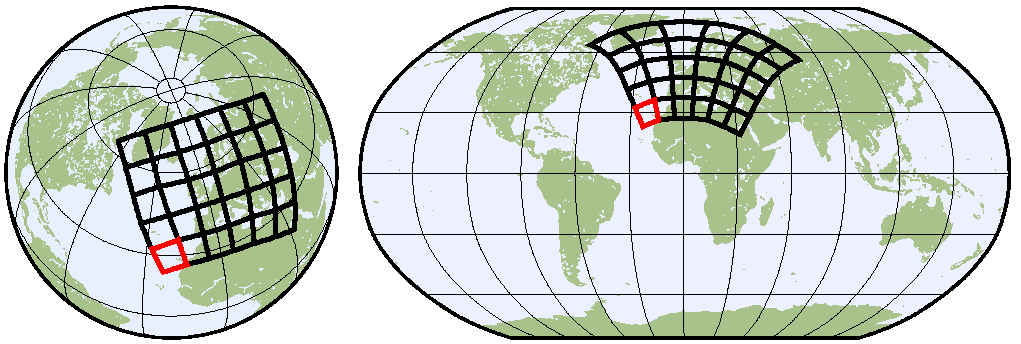
\includegraphics{grids/curv.pdf}}}
}{
{\scalebox{0.99}{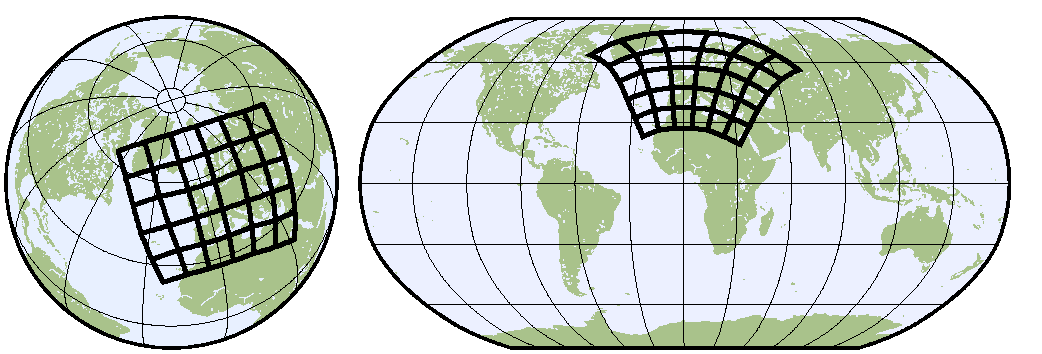
\includegraphics{grids/curv}}}
}
\caption[curvgrid]{Orthographic and Robinson projection of the
  curvilinear grid,  the first grid cell is colored red}
\end{figure}

\newpage
\section{Example description for an unstructured grid}
Here is an example of the {\CDO} description for an unstructured grid.
xvals/yvals describes the position of 30 independent hexagonal grid cells.
The first 6 values of xbounds/ybounds are the corners of the first
grid cell. The first grid cell is colored red.
\begin{lstlisting}[frame=single, backgroundcolor=\color{pyellow}, basicstyle=\footnotesize]
gridtype  = unstructured
gridsize  = 30
nvertex   = 6
xvals     =  |-36|   36    0  -18   18  108   72   54   90  180  144  126  162 -108 -144 
            -162 -126  -72  -90  -54    0   72   36  144  108 -144  180  -72 -108  -36 
xbounds   =  |339    0    0  288  288  309|        21   51   72   72    0    0
               0   16   21    0  339  344       340    0   -0  344  324  324
              20   36   36   16    0    0        93  123  144  144   72   72
              72   88   93   72   51   56        52   72   72   56   36   36
              92  108  108   88   72   72       165  195  216  216  144  144
             144  160  165  144  123  128       124  144  144  128  108  108
             164  180  180  160  144  144       237  267  288  288  216  216
             216  232  237  216  195  200       196  216  216  200  180  180
             236  252  252  232  216  216       288  304  309  288  267  272
             268  288  288  272  252  252       308  324  324  304  288  288
             345  324  324   36   36   15        36   36  108  108   87   57
              20   15   36   57   52   36       108  108  180  180  159  129
              92   87  108  129  124  108       180  180  252  252  231  201
             164  159  180  201  196  180       252  252  324  324  303  273
             236  231  252  273  268  252       308  303  324  345  340  324
yvals     =   |58|   58   32    0    0   58   32    0    0   58   32    0    0   58   32 
               0    0   32    0    0  -58  -58  -32  -58  -32  -58  -32  -58  -32  -32 
ybounds   =   |41   53   71   71   53   41|        41   41   53   71   71   53
              11   19   41   53   41   19       -19   -7   11   19    7  -11
             -19  -11    7   19   11   -7        41   41   53   71   71   53
              11   19   41   53   41   19       -19   -7   11   19    7  -11
             -19  -11    7   19   11   -7        41   41   53   71   71   53
              11   19   41   53   41   19       -19   -7   11   19    7  -11
             -19  -11    7   19   11   -7        41   41   53   71   71   53
              11   19   41   53   41   19       -19   -7   11   19    7  -11
             -19  -11    7   19   11   -7        11   19   41   53   41   19
             -19   -7   11   19    7  -11       -19  -11    7   19   11   -7
             -41  -53  -71  -71  -53  -41       -53  -71  -71  -53  -41  -41
             -19  -41  -53  -41  -19  -11       -53  -71  -71  -53  -41  -41
             -19  -41  -53  -41  -19  -11       -53  -71  -71  -53  -41  -41
             -19  -41  -53  -41  -19  -11       -53  -71  -71  -53  -41  -41
             -19  -41  -53  -41  -19  -11       -19  -41  -53  -41  -19  -11
\end{lstlisting}

\begin{figure}[b]

\ifpdfoutput{
{\scalebox{1}{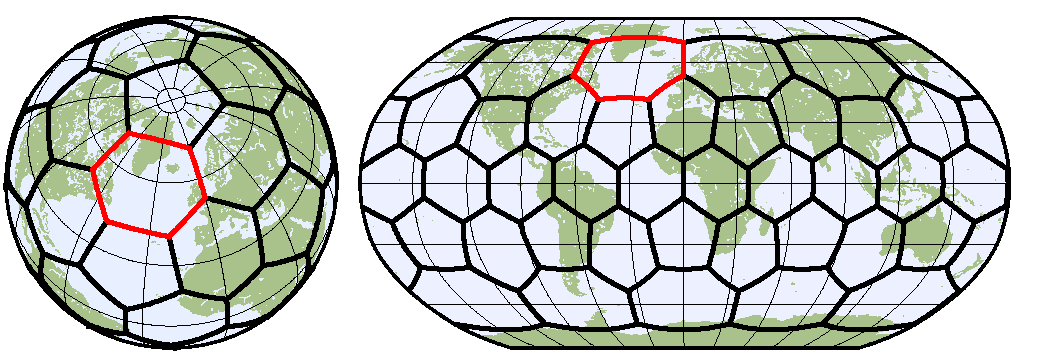
\includegraphics{grids/cell.pdf}}}
}{
{\scalebox{1}{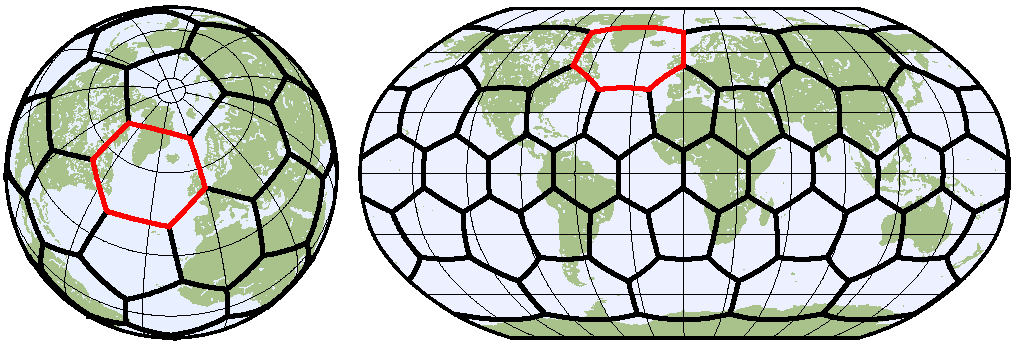
\includegraphics{grids/cell}}}
}
\caption[cellgrid]{Orthographic and Robinson projection of the unstructured grid}
\end{figure}

%%% Local Variables: 
%%% mode: latex
%%% TeX-master: "grid"
%%% End: 


\clearpage
\ifpdfx
\phantomsection
\addcontentsline{toc}{chapter}{\indexname}
\printindex
\else
\input{catalog}
\input{alphabetic_list}
\fi
\end{document}
